\newpage
\section{Results}
\subsection{Experimental Setup}
Executing the MapReduce workflow with different inputs, and configurations:
\begin{itemize}
  \item \textbf{Input size}: the size of the input file is varied to evaluate the performance of the MapReduce workflow.
        \begin{itemize}
          \item \textbf{Paradise Lost} $\sim$ 310 kb
          \item \textbf{Moby Dick} $\sim$ 421kb
          \item \textbf{Frankenstein} $\sim$ 440 kb
          \item \textbf{Divina Commedia} $\sim$ 600 kb
          \item \textbf{Gerusalemme Liberata} $\sim$ 691 kb
          \item \textbf{Promessi Sposi} $\sim$ 1.440 kb
          \item \textbf{Test file} (random generated sequence of char) of $\sim$ 800 Mb.
        \end{itemize}
  \item \textbf{Number of mappers}: Hadoop handles this step
  \item \textbf{Number of reducers}: From one up to three reducers are used for letter frequency
\end{itemize}

\subsection{Performance Evaluation}
\begin{figure}[H]
  \centering
  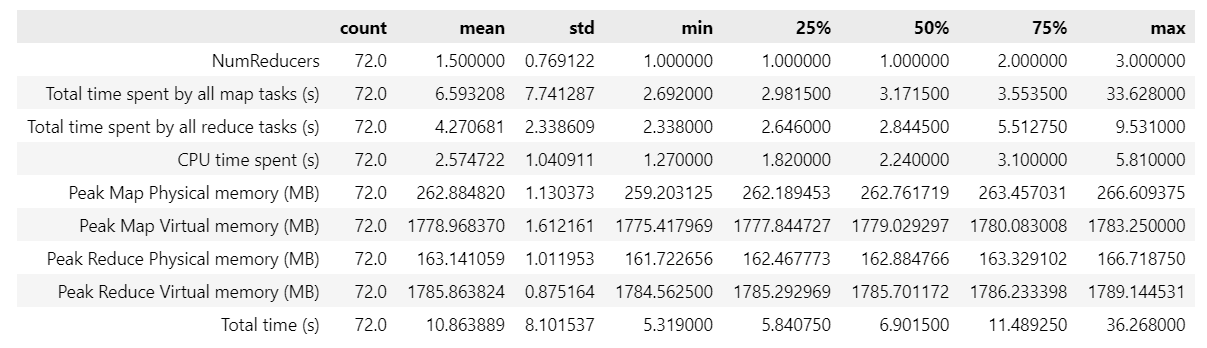
\includegraphics[width=\textwidth]{media/performance/opera_df_describe.png}
  \caption{Statics' insights on Operas}
  \label{fig:OperaInsights}
\end{figure}

\begin{figure}[H]
  \centering
  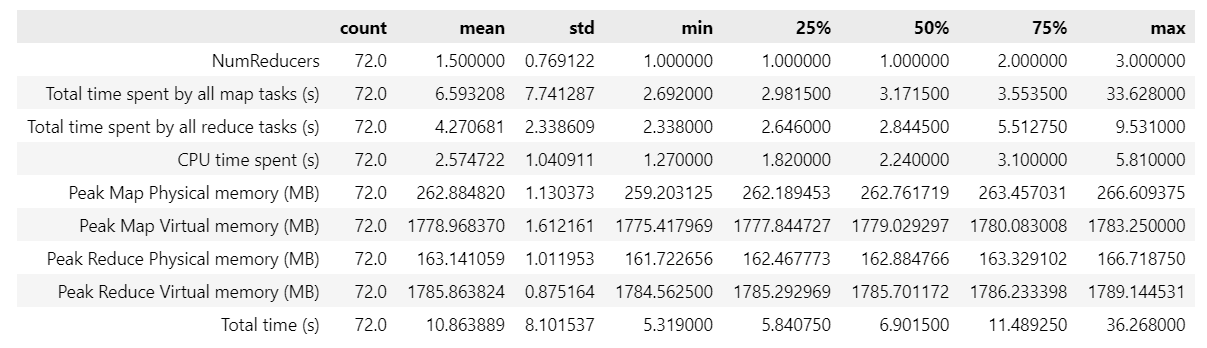
\includegraphics[width=\textwidth]{media/performance/opera_df_describe.png}
  \caption{Statics' insights on Test}
  \label{fig:OperaInsightsTEST}
\end{figure}


\begin{figure}[H]
  \centering
  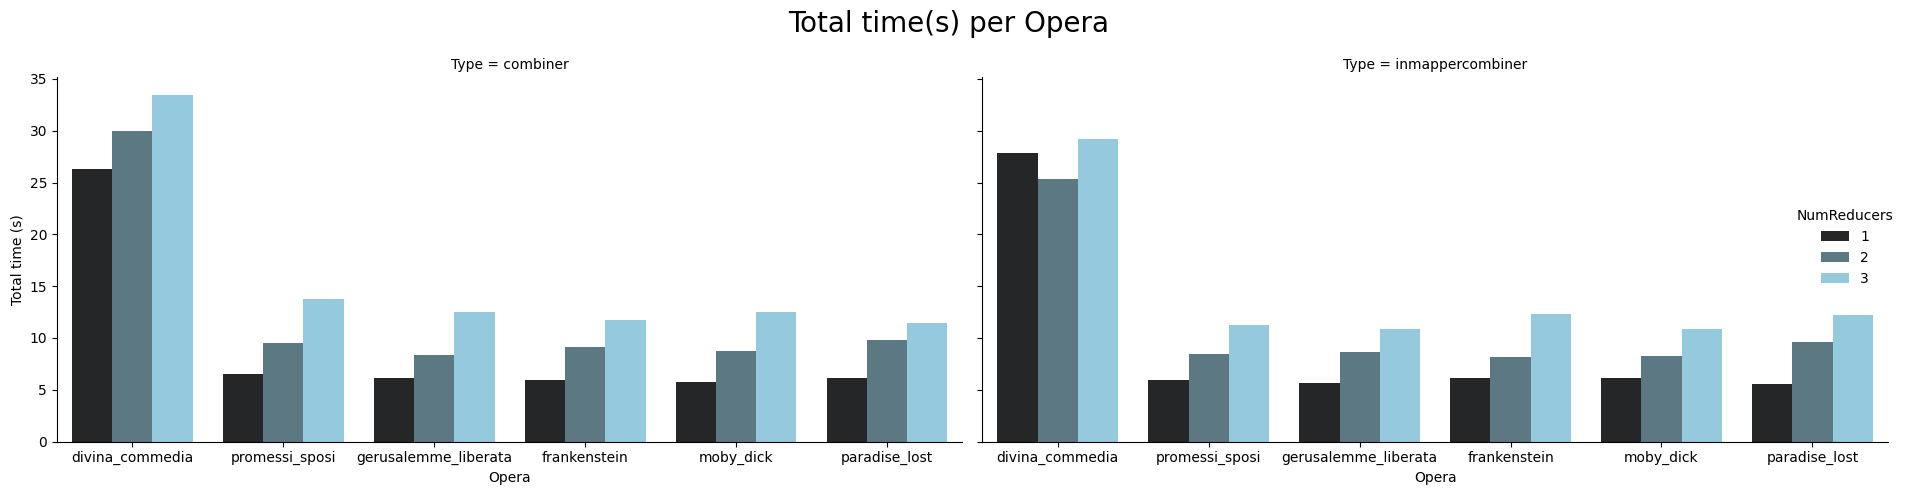
\includegraphics[width=0.8\textwidth]{media/performance/total_time_S_per_opera.png}
  \caption{Total time for each opera with different reducers}
  \label{fig:TimeOperas}
\end{figure}

\begin{figure}[H]
  \centering
  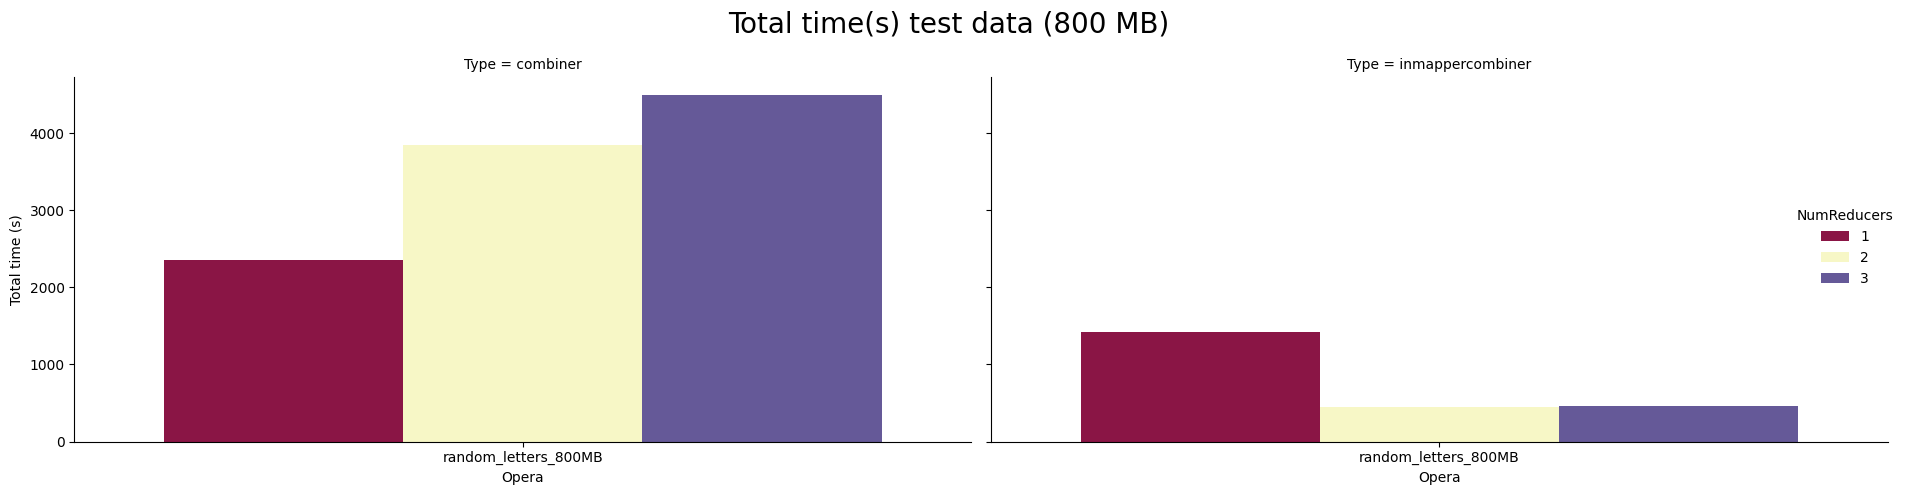
\includegraphics[width=0.8\textwidth]{media/performance/total_time_S_per_opera(TEST).png}
  \caption{Total time for Test with different reducers}
  \label{fig:TimeTest}
\end{figure}

\begin{figure}[H]
  \centering
  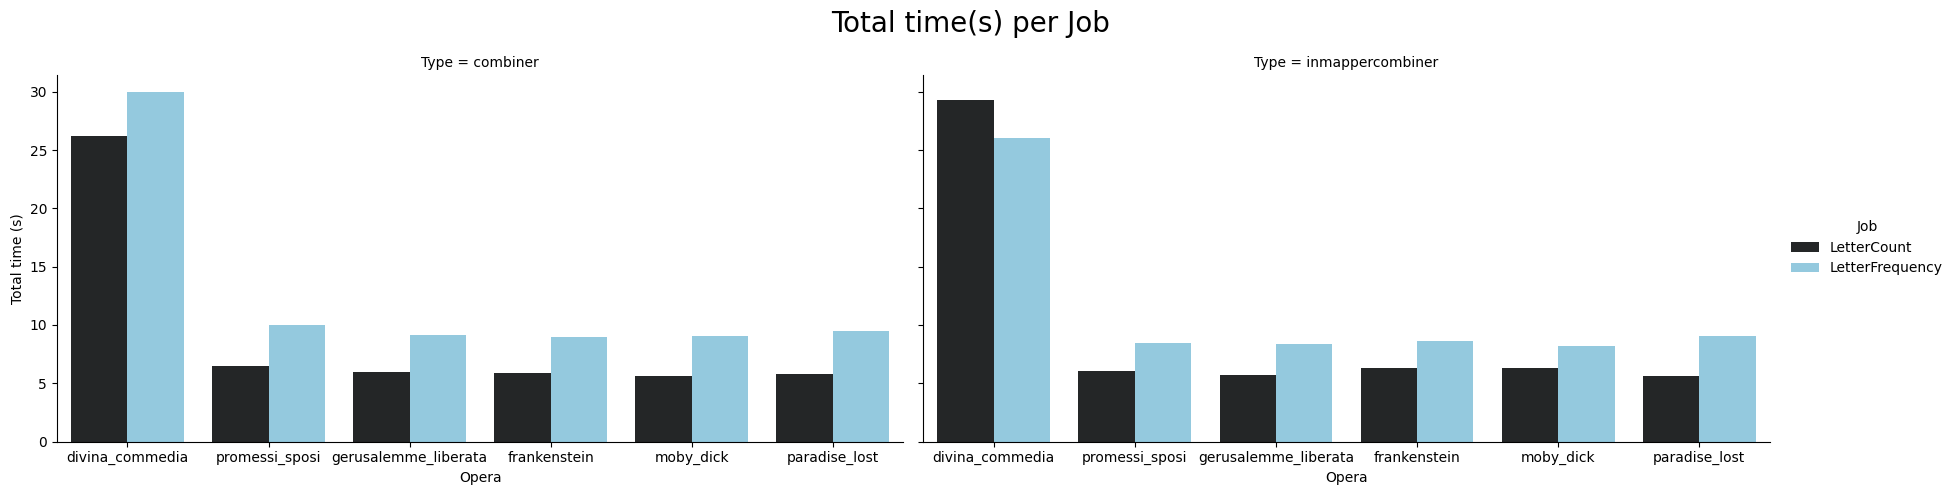
\includegraphics[width=0.8\textwidth]{media/performance/total_time_S_per_job.png}
  \caption{Total time for each job with different operas}
  \label{fig:TimeJob}
\end{figure}

\begin{figure}[H]
  \centering
  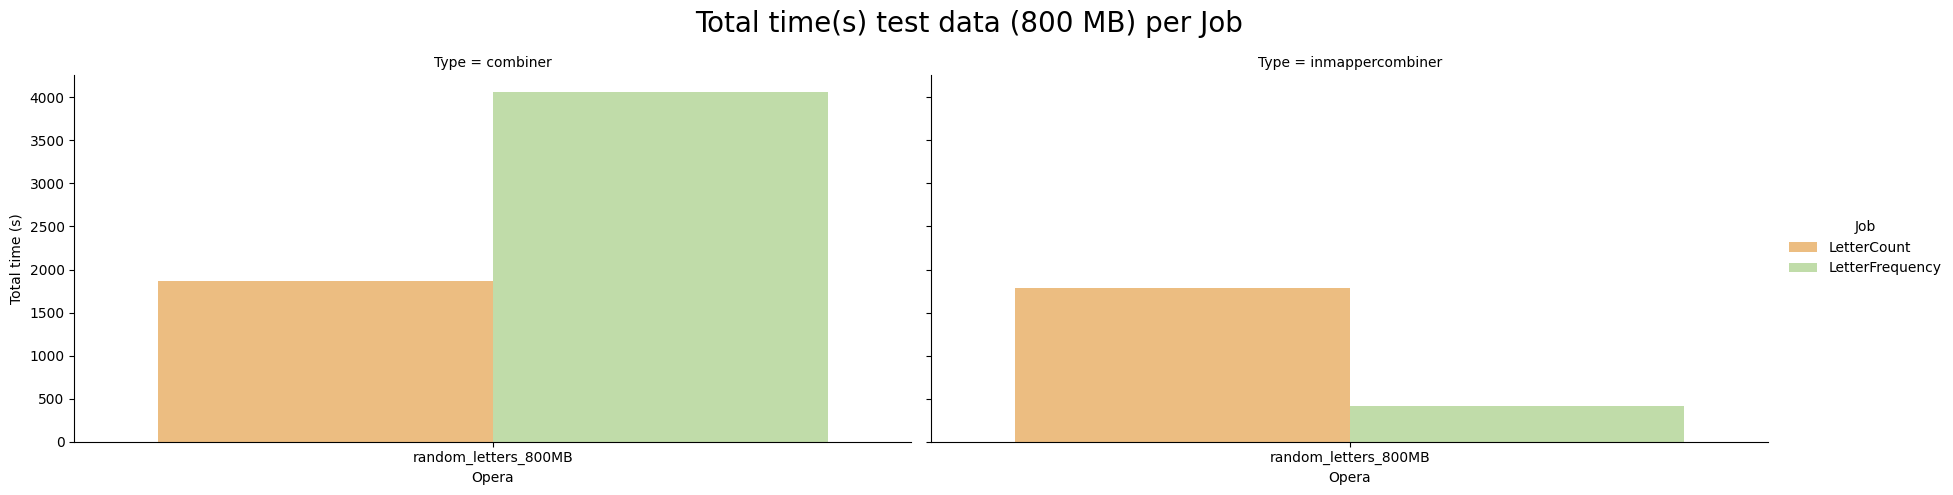
\includegraphics[width=0.8\textwidth]{media/performance/total_time_S_per_job(TEST).png}
  \caption{Total time for each job with Test}
  \label{fig:TimeJobTest}
\end{figure}

\begin{figure}[H]
  \centering
  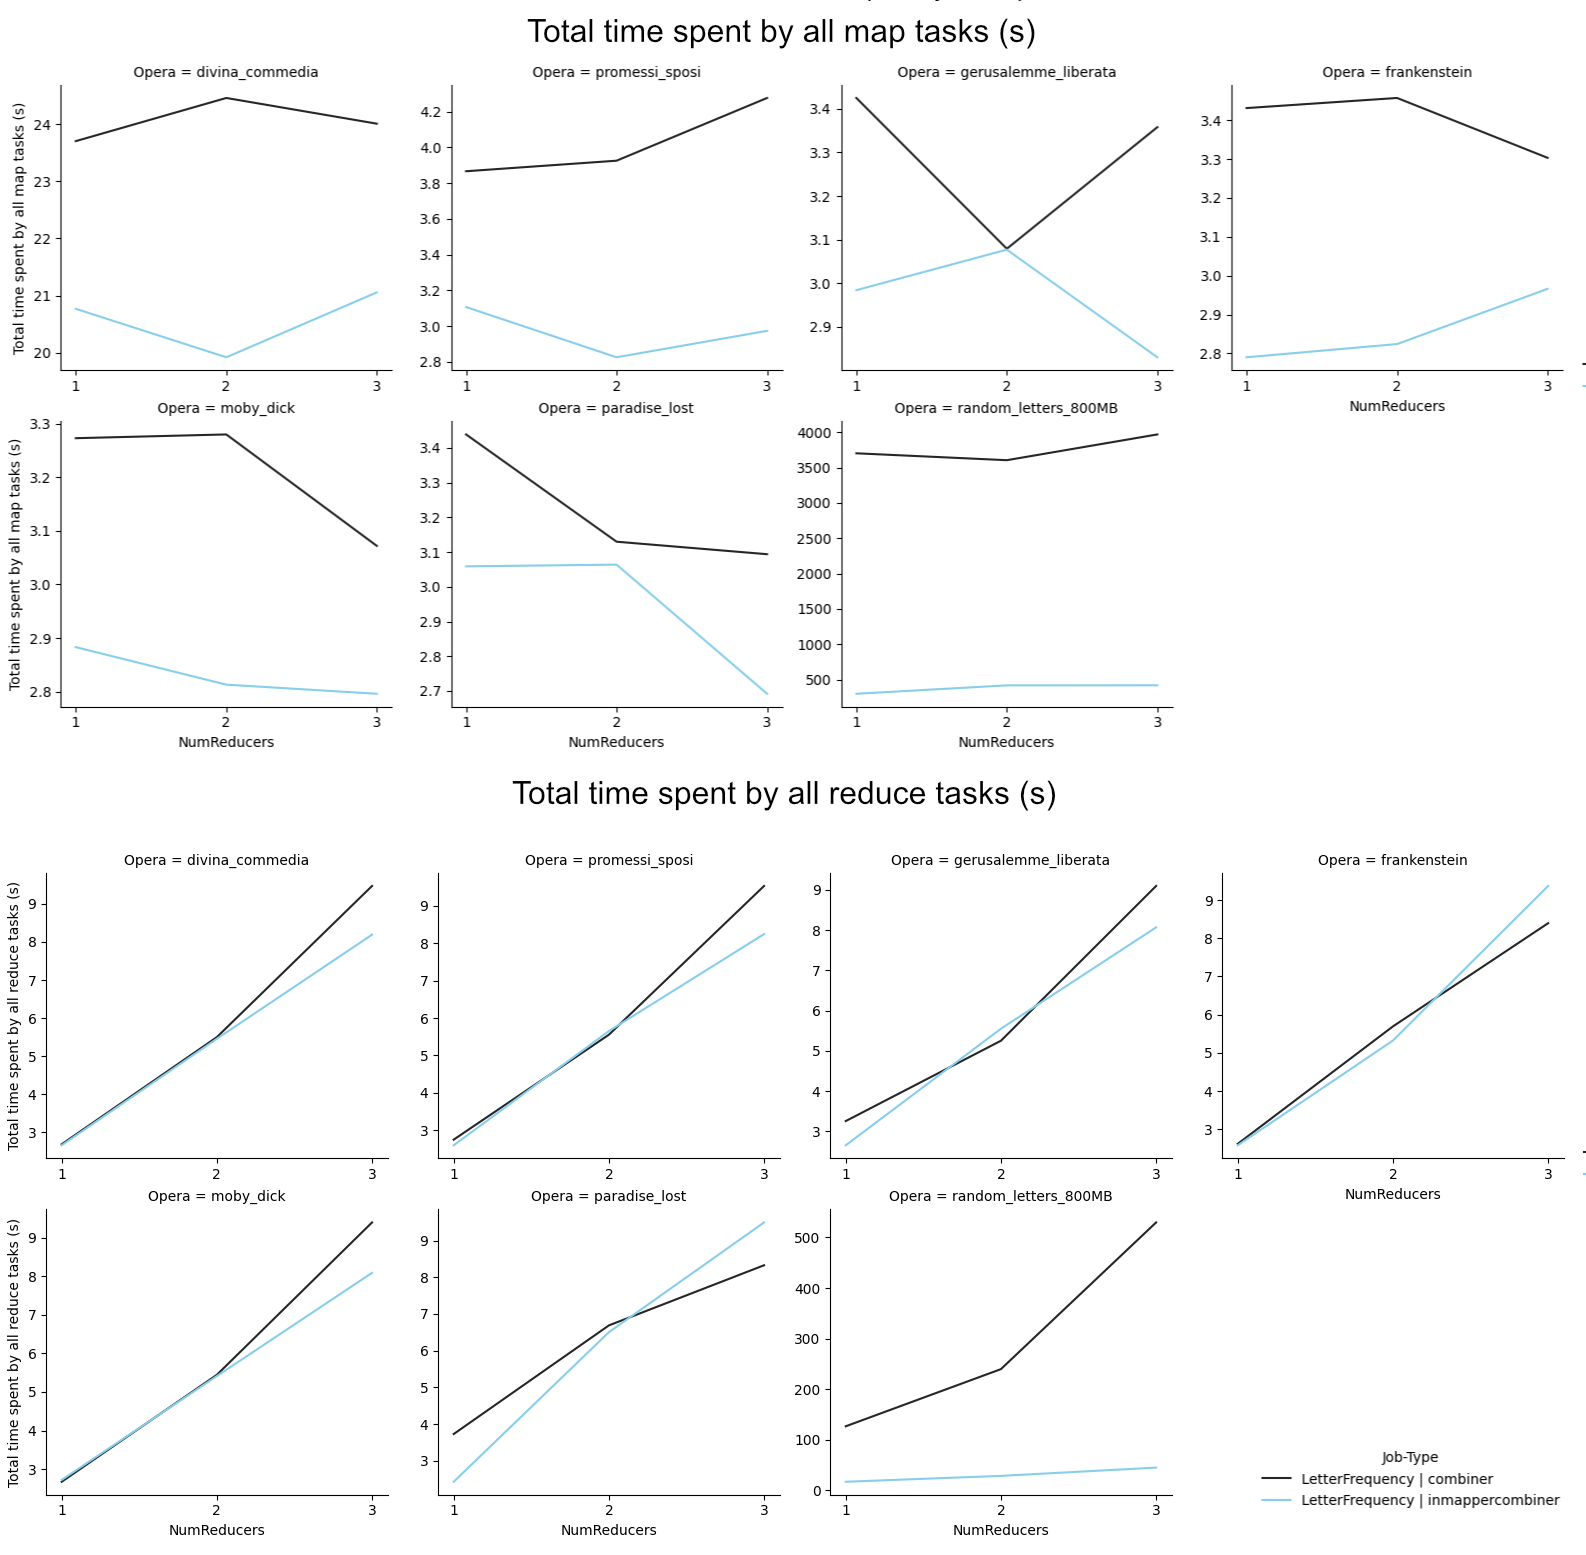
\includegraphics[width=0.8\textwidth]{media/performance/TotalTimeMapReduce.png}
  \caption{TotalTimeMapReduce}
  \label{fig:TotalTimeMapReduce}
\end{figure}

\begin{figure}[H]
  \centering
  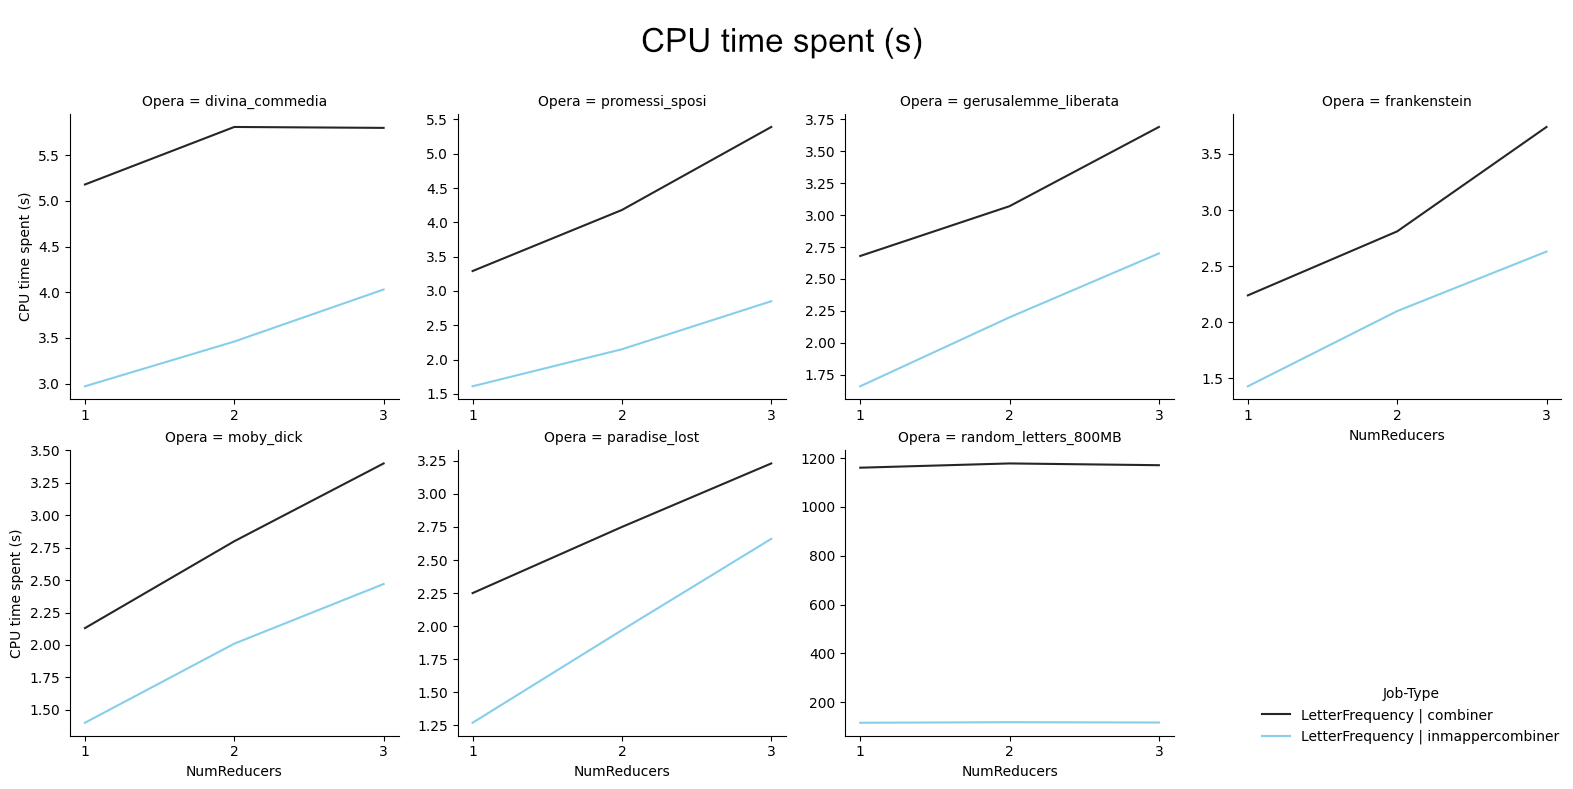
\includegraphics[width=0.8\textwidth]{media/performance/CpuTIME.png}
  \caption{Cpu Time}
  \label{fig:CpuTIME}
\end{figure}

\begin{figure}[H]
  \centering
  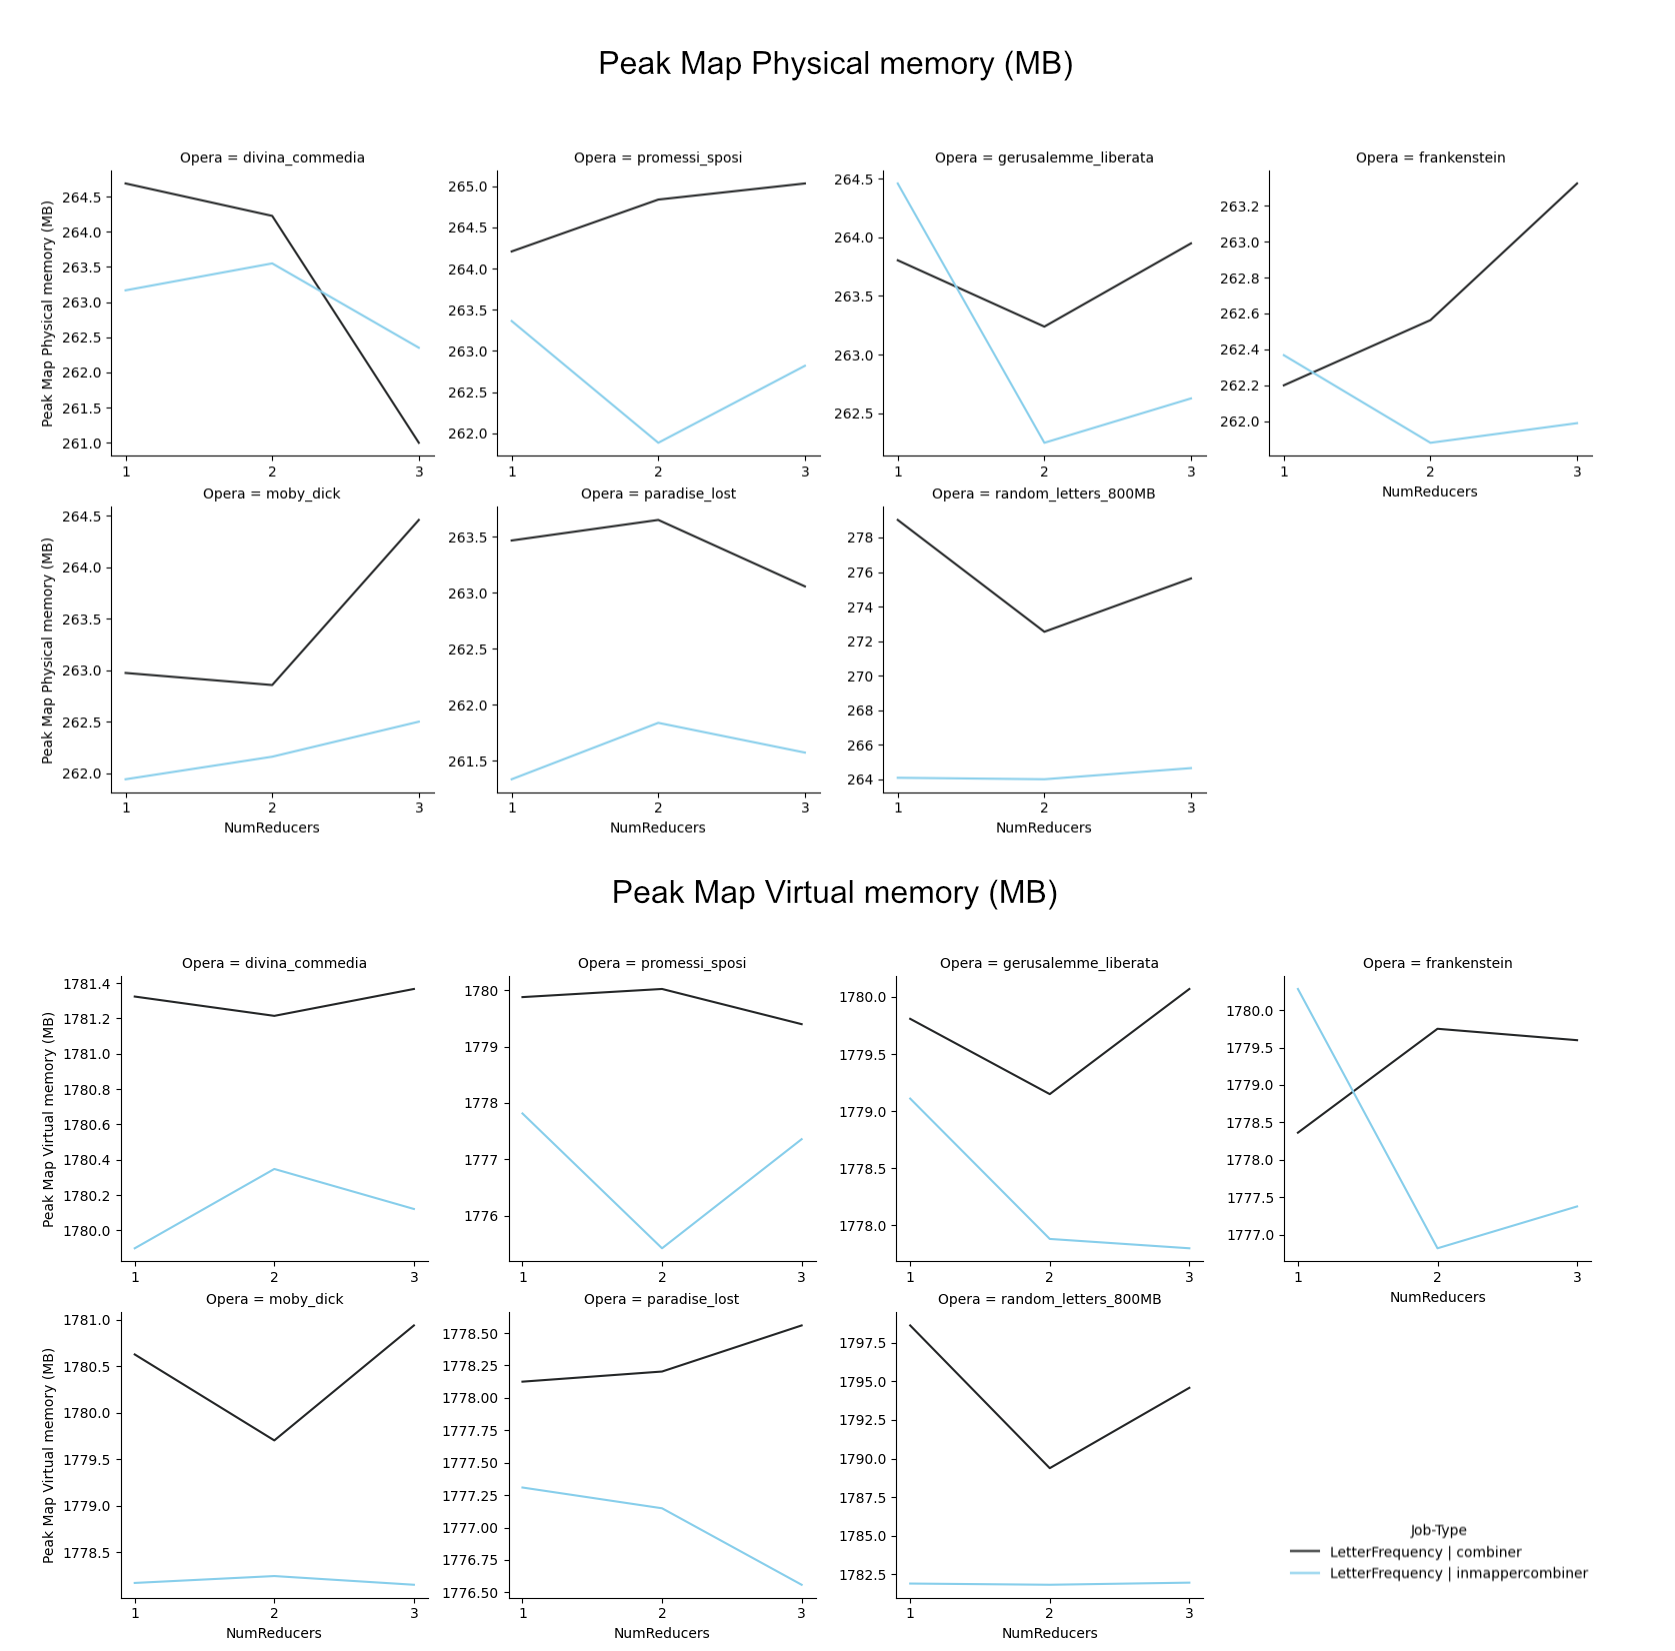
\includegraphics[width=0.8\textwidth]{media/performance/PeakMapMemory.png}
  \caption{Peak Map Memory}
  \label{fig:PeakMapMemory}
\end{figure}

\begin{figure}[H]
  \centering
  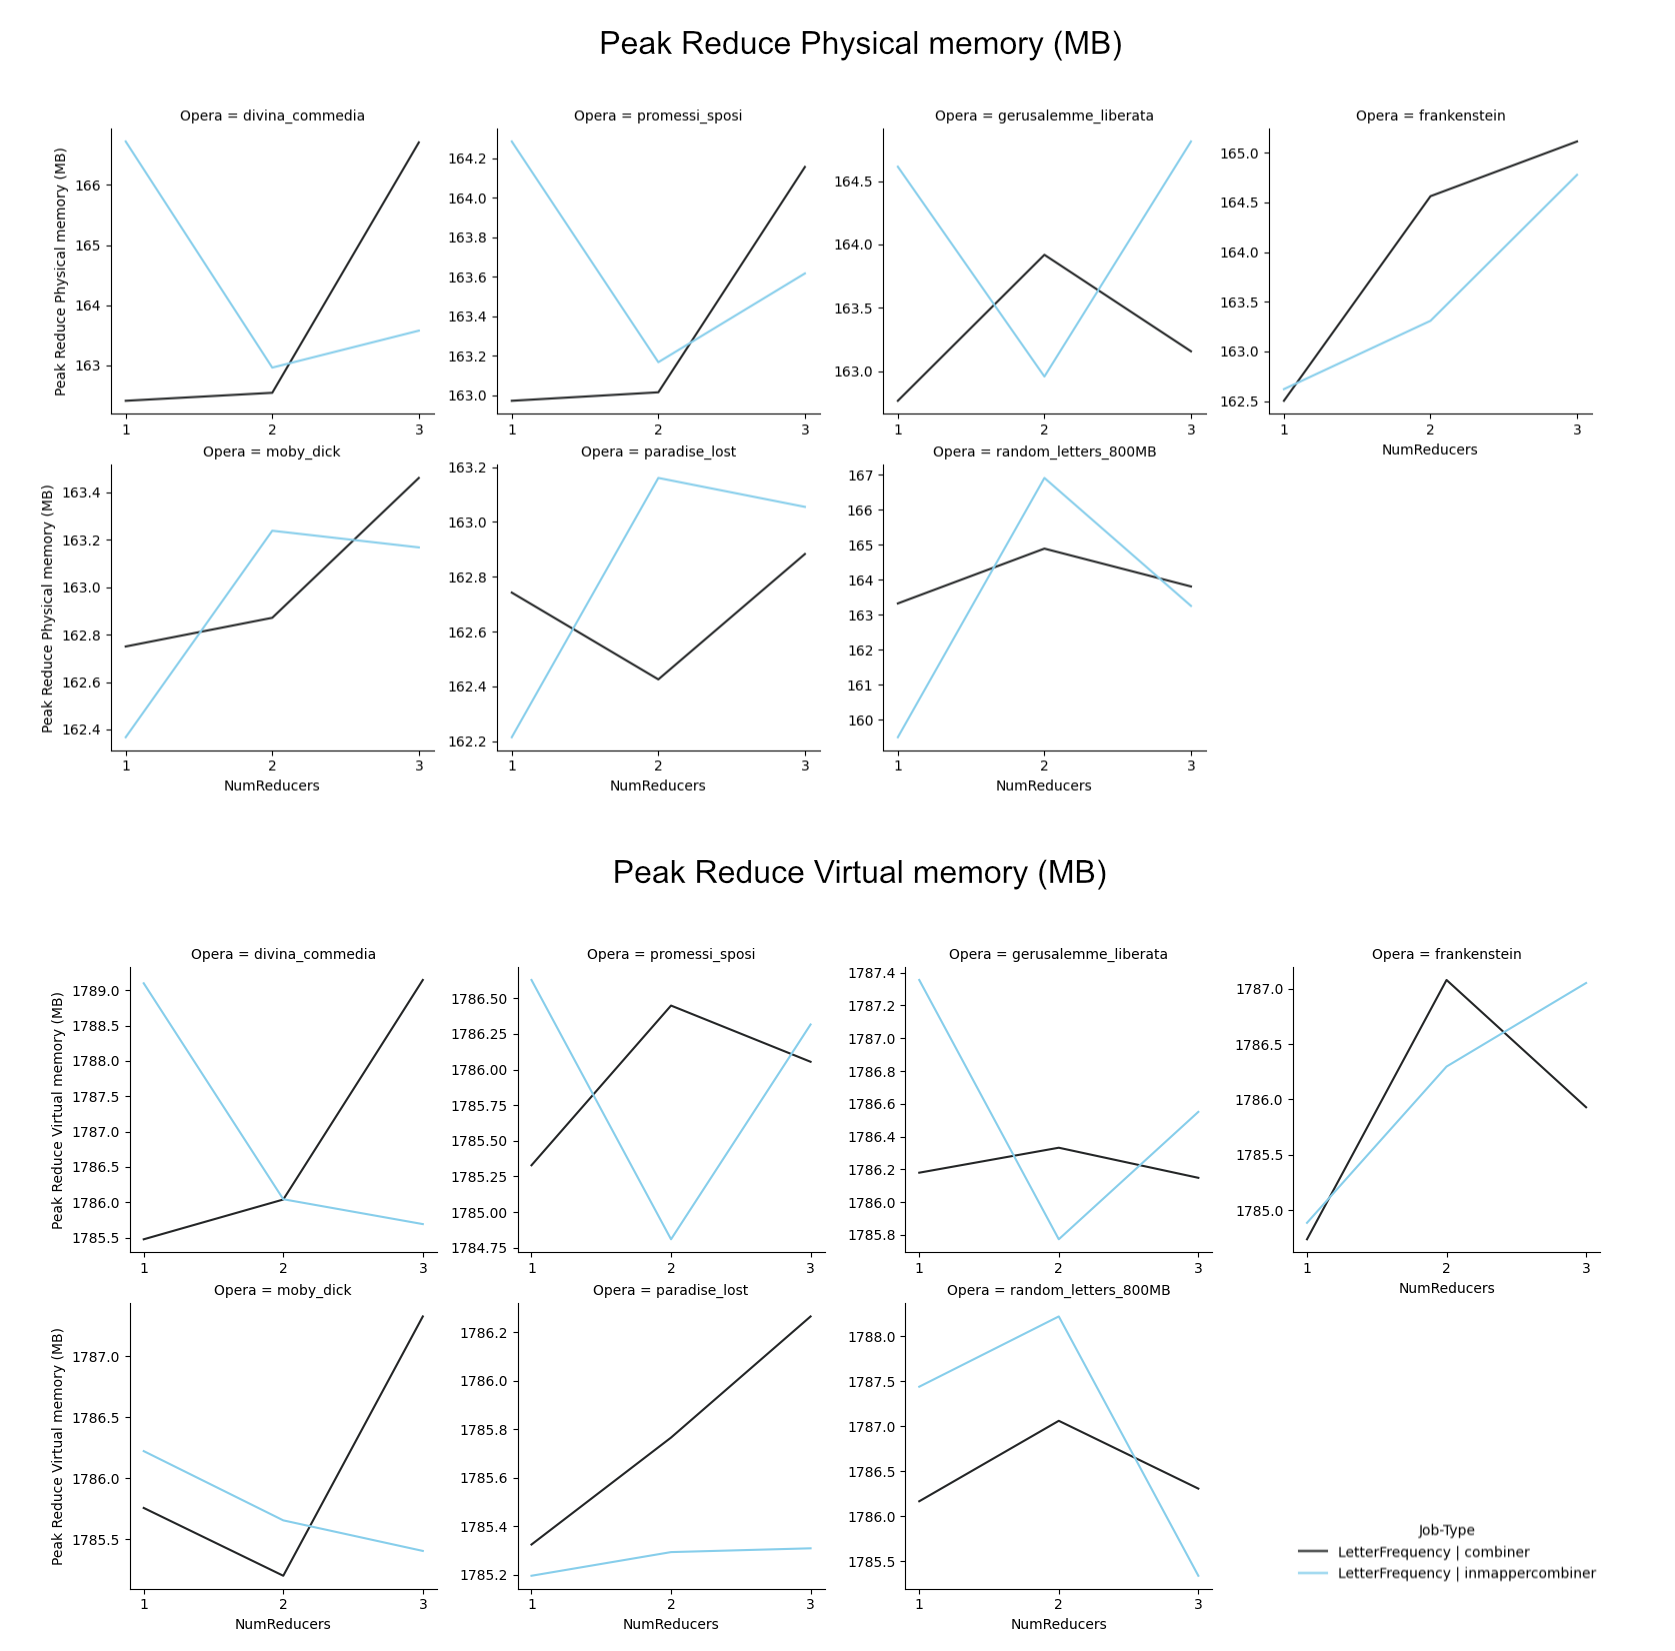
\includegraphics[width=0.8\textwidth]{media/performance/PeakReduceMemory.png}
  \caption{Peak Reduce Memory}
  \label{fig:PeakReduceMemory}
\end{figure}

\subsection{Local Python script comparison}
As expected, the execution of a local Python script showed excellent performance with small text sizes. In these cases, the absence of the map and reduce phases, typical of the Hadoop framework, proved advantageous. For smaller files, these phases can even be counterproductive, increasing execution time due to the overhead introduced by the distribution and management of tasks among the cluster nodes.

\noindent However, for large files, Hadoop demonstrated significantly better performance compared to the local Python script. Hadoop's ability to distribute the workload across multiple cluster nodes and efficiently manage large volumes of data resulted in reduced execution times even for substantial datasets, confirming its effectiveness in handling big data.
